%!TEX root = project.tex

\chapter*{Abstract}
For our final year project, we wanted to create an industry standard application based on something that we all loved. In our case this was music. We felt that if we were working on something that we loved it would be more enjoyable than working on something that we didn’t. The basis of our application is a personalised playlist creator which also has the capability of merging your playlist with a friend to create a playlist with both of your preferred music in it. We felt this was a fantastic idea as when the three of us would go in the car together none of use could agree on music to liston to ,  perhaps if we had an app like this during the journeys , all of the music arguments we had wouldn’t have happened. The main goal of this project was to create a 3 tier application , we used MongoDB as our data tier, Flask and python for our logic tier and React native for our presentation tier. These three tiers gave us the architecture for our application called “WePick”.


\chapter{Introduction}
When we first began to brainstorm ideas for our project, we decided to focus our project on the theme of music. This was an obvious choice for us because its something that the three of us have a keen interest in. At the start we thought of an idea to create our own music player, but soon decided after great research\cite{MusicApps}  that they’re numerous apps like this available and if we did develop this we would just be adding another music player to the app store that probably wouldn’t be used. 
\par
Finally, we thought of the idea of “WePick”, a personalised playlist creator with the ability to create a community playlist with your friends. This seemed like the perfect idea and something that the three of us would regularly use if there was an app like this on the market. Although it was a fantastic idea, we now needed to come up with a development plan. We had decided before the idea of “WePick” that we wanted to create a 3-tier application but were unsure what we would use for the tiers. After about a week of research into different technologies we decided to go with React for the presentation tier. The main reason for this was due to it being top 5 in the most used front-end JavaScript frameworks\cite{Top5Frontend}. Our next choice was what type of database to use for our data layer. This was a tough one because we wanted to be able to easily communicate with our database and be able query our database to send and receive JSON data. For these reasons, we decided to go with the popular MongoDB. For the logic tier we decided to use Python along with Flask for web server. We then decided to use Axios which is a Promise based HTTP client for communication between our database/Flask server and our React front-end.
\par
Using all these technologies we planned to develop an application that was responsive, easy-to-use and overall accomplished our original goal of creating curated playlists based on multiple people's music preferences.



\chapter{Context}
The context of this project revolves around the use case of multiple people sitting together in a car or house and not being able to decide on what music to play. One of the people can open the app and generate a playlist that they all enjoy instead of spending time on deciding what to play specifically.
This person will have had an account registered previously and as long there are other people with them they can all generate playlists of music depending on their preferences.\newline

The goal of our project was to develop a dynamic web application that creates curated playlists based on multiple user's music preferences using Spotify.
The project was completed over a 7-month period and this meant that the project environment didn’t change drastically.

\section{Project Reference}
https://github.com/WePickOrganization/WePick

\section{Objectives}
The project required several objectives to be accomplished in order to provide a solution that worked.
\begin{itemize}
	\item Set up a MongoDB database that will be used to store the user’s preferences along with the user’s email and password.
	\item Host the application in the cloud – using AWS. This must be done so the application can be accessed from any desktop.
	\item Authenticate user credentials through Spotify to give a secure connection.
	\item Develop an intuitive user interface using React, which will serve as the front-end for the application.
	\item Set up a Flask server using Python to serve as a backend for the application.
	\item Use Python along with the SpotifyAPI to generate the playlist using the user’s music preferences.
	\item Allow users to generate a playlist based on different artists.
\end{itemize}

\section{Overview}
Each chapter of this minor dissertation gives different details on this group project.\newline

The Methodology outlines the various development methodologies that were used through out the development of this project such as version control tools, sprints, weekly meetings etc.\newline

The Technology Review discusses in detail, the different technologies that were used throughout the project. Demonstrating the approach to the various technologies and our reasons for choosing them.\newline

The System Design provides the detailed information about the overall architecture of the system whilst also looking at the implementation at a function level.\newline

The System Evaluation section poses the project against the objective and proves robustness and performance of the project through the testing techniques that were used through out development.\newline

The Conclusion will be a reflection on the entire project, whilst discussing any difficulties, learning outcomes and future developments of the application.

\chapter{Methodology}
In this section we do an extensive run through of all the methodologies we used throughout our project. Methodology is the way you plan and control the development process of a piece of software or anything that needs to be developed. There are lots of software methodologies out there like the Waterfall model, Rapid Application Development, Extreme Programming Methodology and Spiral Model. They each have their advantages and disadvantages, but we decided to go with Agile as our methodology for our project. The main reason for this being that many jobs that companies advertise around Ireland use Agile, so we wanted to familiarise ourselves with this methodology for when we enter the job-hunting world.

\section{Agile Development}
When we began to develop our project, we decided to go with an Agile approach for the research, design and implementation stages of our project. As mentioned above, the reason we chose Agile was because of its frequent use in most companies that we applied jobs for. But another major reason for the many advantages Agile offers. These include but are not limited to continual improvement, flexibility and incremental delivery of the software. This was extremely important for us because we were adding important components every week, and this is something Agile allows.
\par
When we were at the research and development stage, we used a scrum like approach which is very common in an Agile environment. Scrum is an Agile methodology which a development cycle is carried out in what are called sprints. Later in the document, I will go through each stage of the sprints in the research and development phase and explain in detail what we went through in those sprints.
\par
During the life cycle of our project, we would hold meetings three times a week. When I say life cycle, I mean the Initiation, Planning, Execution, Closure of our project. During these meetings we would discuss what features we had working in our projects and what features we planned to start developing in the following week. We would also meet with our project supervisor once a week to discuss our plans for the next week just to keep him updated on our progress throughout our project and to resolve any issues we might have encountered. Before each sprint in our project, we used these meetings to plan our sprint cycle which usually lasted around two weeks. 
\par
To help us keep track of our sprint plans we used GitHub’s project page. This page was vital for us because it allowed us to add tasks to different lists. These lists include to-do, in-progress and done. Once we thought of something to add or improve at our weekly meetings we added these to the to-do list, then when we were ready to start the task we would add that to our in-progress list, finally when we finished that we added it to the completion list. This proved very important to us because it allowed us to keep track of what we had to do and what we had done already. It was also a plus to be able to look back at how much progress we had completed.
\begin{figure}[ht]
\renewcommand\thefigure{3.1}
\centering
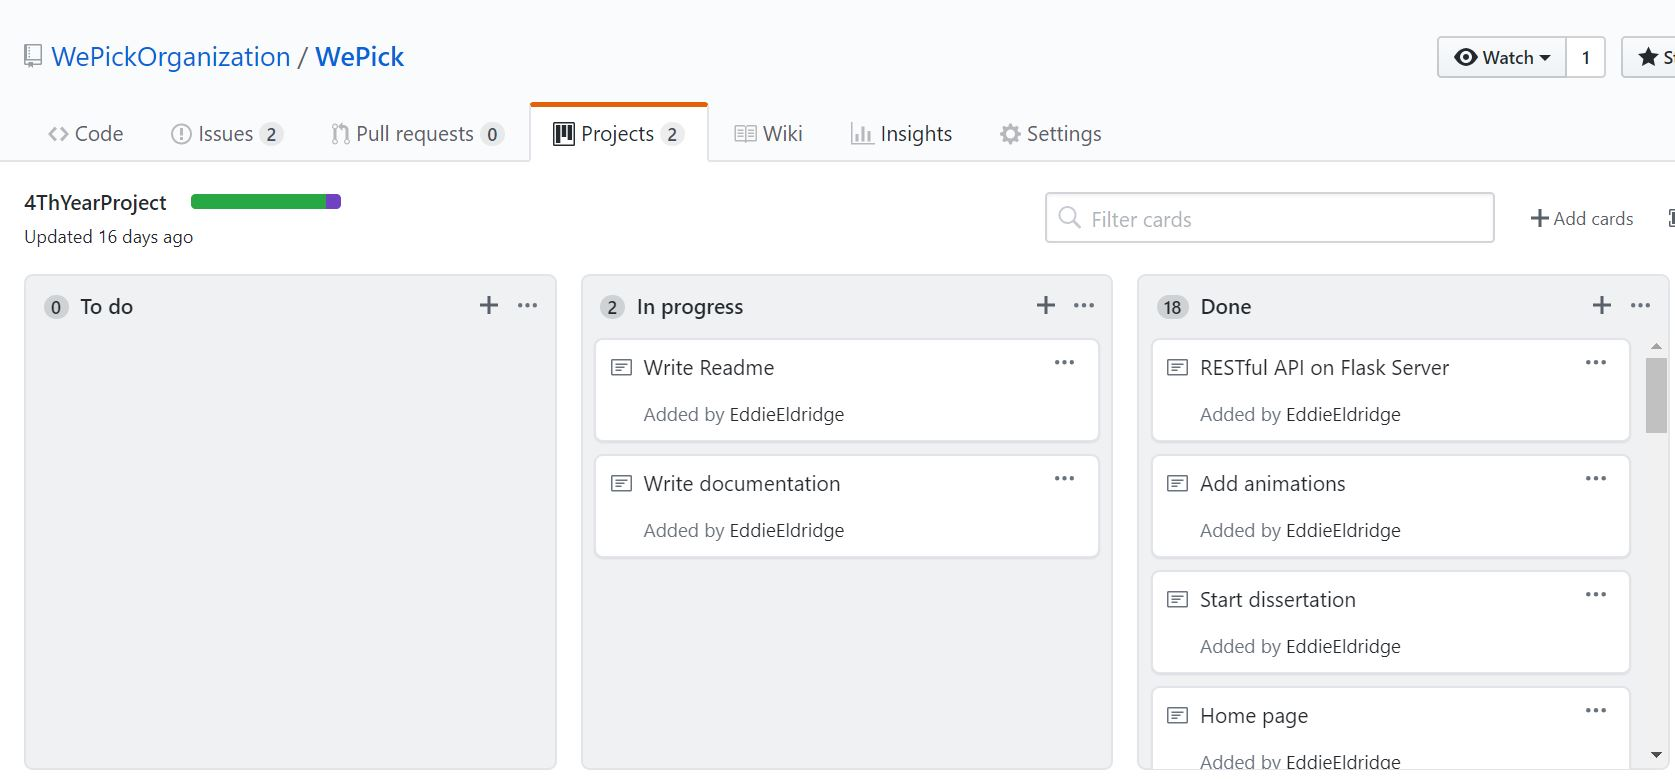
\includegraphics[width=14cm, height=8cm]{img/projectboard.JPG},
\caption{Git Project}
\label{Github Projects}
\end{figure}
\par
We found our meetings with our project supervisor extremely helpful because although we were having frequent meetings by ourselves, it was very handy to be able to iron out issues that we had and to just make sure we were going on the right track with the guidance of Martin at the end of every week.

\section{Version Control}
Throughout the life-cycle of our project, we used GitHub which is a web-based hosting service for version control using git. Git itself is a version-control system for tracking changes in source code during software development. Its focus is to allow collaboration between developers on a single project, but it can be used also to track changes in any set of files. We found GitHub to be extremely helpful when developing our project because it allowed all three of us to work on the project together. We did this by setting up branches for each of us and when we began to test features, this allowed us to , in case it didn’t work. We then merged the branches to the master when we were confident that the merge wouldn’t cause conflicts in the working code. This was our first-time using branches for our projects and after using them, we can clearly see that branches are essential for testing features without touching the working code on the main branch. Aside from version control, as mentioned above, we also used GitHub’s project tab to keep track of the tasks we must do, tasks we were currently doing and tasks that we planned to. We found this to be helpful as it allowed us to break a big project into small tasks. Along with these, we found it very easy to revert to a previous commit in case an issue arrived that we couldn’t fix. This happened quite a bit throughout our project.
\begin{figure}[ht]
\renewcommand\thefigure{3.2}
\centering

\includegraphics[width=13cm, height=5cm]{img/github.png},
\caption{Github}
\label{Github VC}
\end{figure}\\



\newpage\subsection{Travis CI}
Travis CI is a hosted, distributed continuous integration service used to build and test software projects hosted at GitHub. The way this works is that it runs your program's tests every time you commit to GitHub (this can be configured in many ways, and you can always disable builds on some branches). The advantages of this is that you can often discover very quickly if your commit broke something and fix it before it becomes a problem. This was very useful for us as it allowed us to see the errors rather then not knowing. This then allowed us to fix the issue before the next commit. 

\begin{figure}[ht]
\renewcommand\thefigure{3.3}
\centering
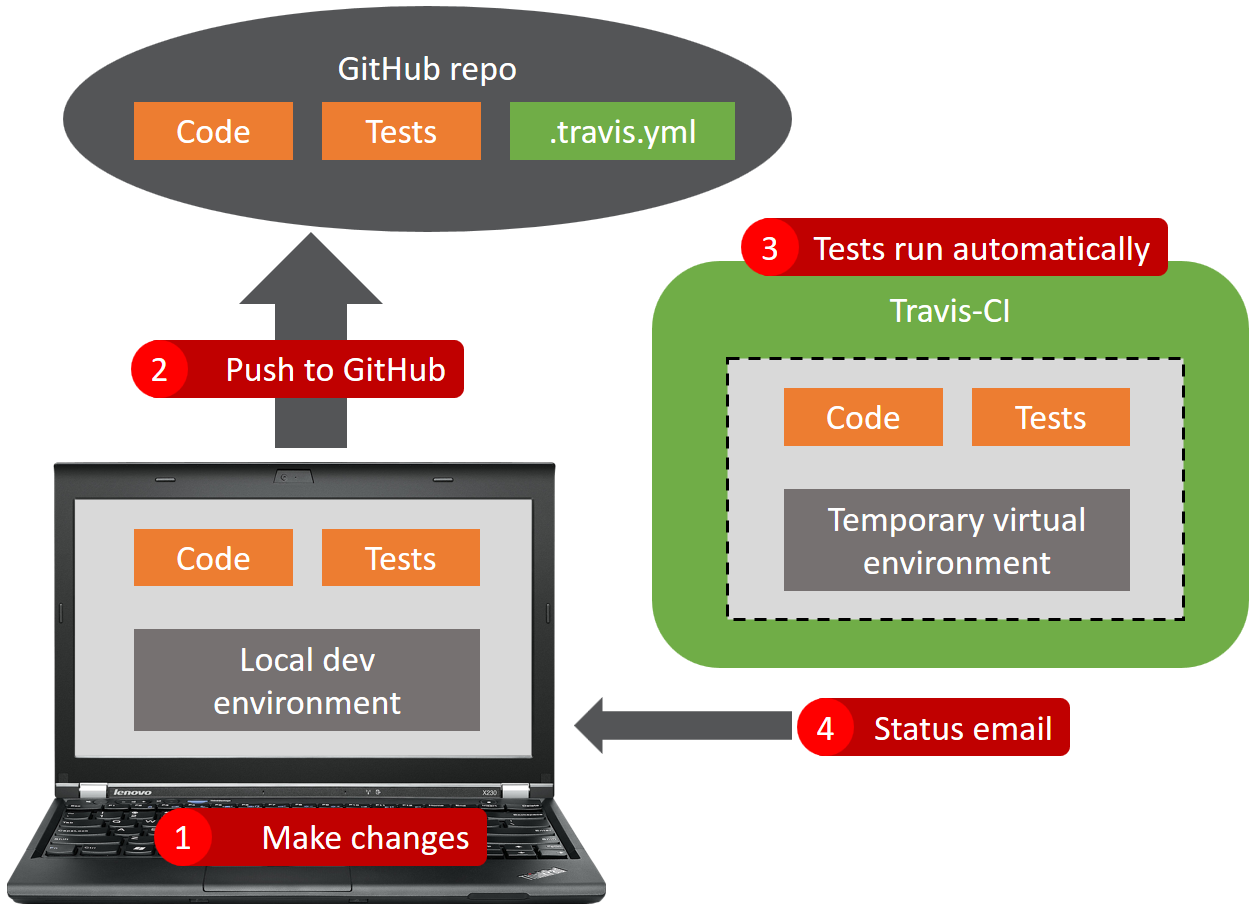
\includegraphics[width=10cm, height=7.5cm]{img/travis.png},
\caption{Travis CI}
\label{TravisCI}
\end{figure}

\subsection{Whitebox Testing}
White box testing is a software testing method in which the internal structure/design/implementation of the item being tested is known to the tester. During the life cycle of our project we did a lot of white box testing. This included testing a lot of the input fields to see if it would accept illegal characters or text that wasn’t in the right format for the input. One we took caution when testing was the log-in/register as we wanted to make sure that the user could only enter an email for the email field. In the beginning we knew this wasn’t going to work but then we added in some simple functions that checked wither the string had an ‘@’ symbol and also contained a ‘.’. These two conditions are a good way of checking if a user has entered a valid email or not. A major advantage of white box testing was that we were able to test inputs earlier in the development process as we didn’t need a GUI which took a long time by itself to create. This however wouldn’t be suitable as a black box test as the user shouldn’t know how to test the code using the command line and only using a GUI with well written instructions.

\begin{figure}[ht]
\renewcommand\thefigure{3.4}
\centering
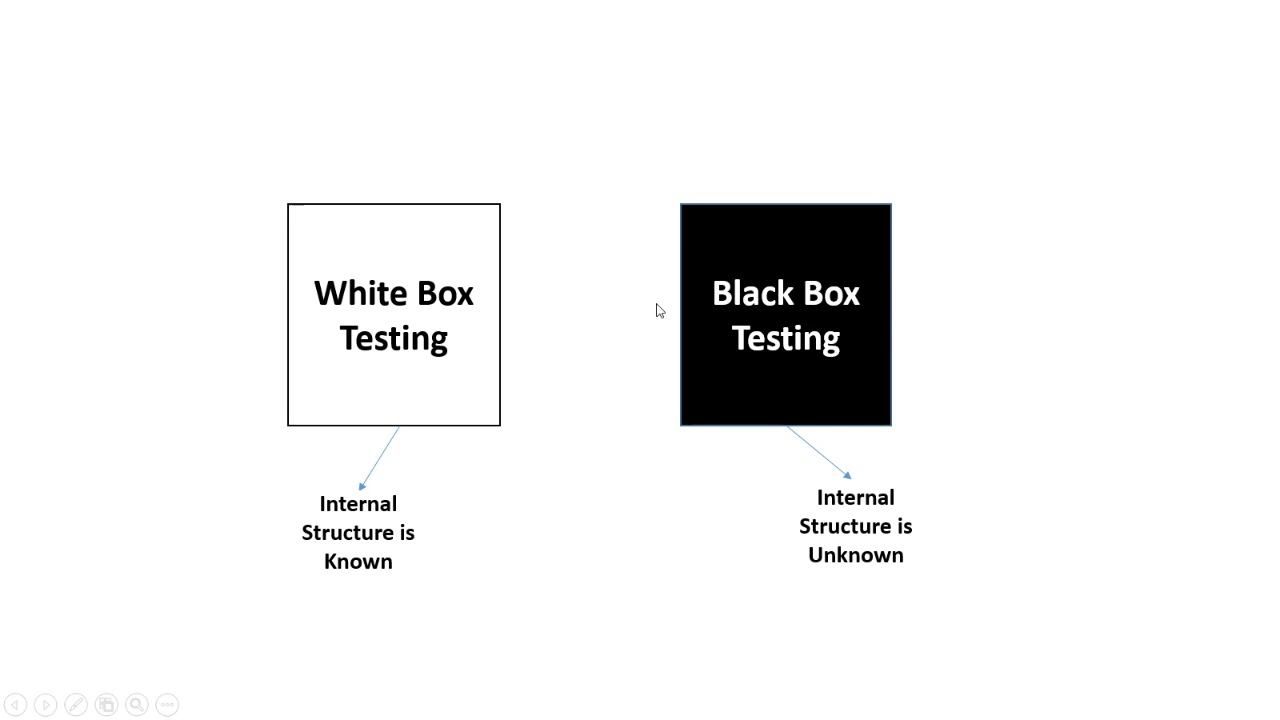
\includegraphics[width=10cm, height=5cm]{img/whitebox.jpg},
\caption{Whitebox vs Blackbox Testing}
\label{whiteboxvblackbox}
\end{figure}

\subsection{Blackbox Testing}
Black box testing, also known as Behavioural Testing, is a software testing method in which the internal structure/design/implementation of the item being tested is not known to the tester. This is sometimes a better approach to testing as the tester can test the system as they please in contrast to a developer where they sometimes test a system gently to keep the system working. We also used a lot of black box testing towards the end of our project. We let random students in our class test different components of our application and recorded the result. With this type of testing we were extremely interested to see how a regular user would navigate our application and if they would face problems. One interesting observation we saw was that sometimes when registering a user may incorrectly enter the ‘@’ character with the ‘ ‘ ‘ character when entering the email. This was something we hadn’t spotted before and then began to implement string checks on the input of emails. This was something we may not have spotted with white box testing as we may have only entered valid emails because we assumed that an end user would never make mistakes. This however, we found to be false as everyone makes mistakes.
\\
\\
\\
The following two sections contain information about the various sprints we undertook in the research.

\section{Sprints} 
In this section we will discuss more about sprints. A sprint is a short, time-boxed period (Usually about 1-2 weeks for us) where a scrum team works to complete a set amount of work. Sprints help teams follow the Agile principle of "delivering working software frequently". As I discussed earlier, we used sprints throughout the whole life cycle of the project. Every sprint we completed in the research phase of the project allowed us the opportunity to come together as a team and learn more about the various components needed for our application. During the development stage, each sprint brought us one step closer to having a fully completed project.

\section{Research Sprints}
\subsection{Sprint 1: Initial Research}
Our first sprint was based on initial research of the project. We wanted to research the technologies needed to create the application. We first decided on researching databases and quickly decided to go with MongoDB as it would allow us to work with a lot of non-structured data. Before beginning, we also decided we would use Python to write our application as we all were familiar with the syntax and enjoyed it as a programming language. Finally, we decided to go with React as our front-end framework as it is a very popular framework. We also choose it because a lot of web development companies use React, and we wanted to be familiar with how it worked.

\subsection{Sprint 2: Review}
When we finished the first sprint, we wanted to create a diagram which showed how all three technologies were connected. We felt this was essential to make sure all of us were sure of how we would be developing the application and that nobody was confused. During this sprint we each took turns explaining to each other how the project worked. We also made a simple flow chart with how we thought the user would interact with our system.

\subsection{Sprint 3: Front-End design and database design}
For the design of our front end, we wanted to make it very simplistic with a dark theme of colours. We decided this by visiting our favourite websites and deciding what we liked and didn’t like about the design. We then wrote down all the things we liked and based our design of these points. From here, we sketched out a simple homepage and other components. This allowed us to get a real taste of how the application would look a few months down the line. After we completed this we sketched out the different attributes we needed for our database and built a simple table. We decided we would work more on the database down the line but just wanted to have a simple table to test on.

\section{Development Sprints}
\subsection{Sprint 1: Flask app connected to database}
When we began writing the application, we based our development of a sample flask app we found online. Although we used nothing from this, we used it to understand how everything worked. From here we then began to connect the flask app to our database using the PyMongo libraries. We set up simple functions to add/select/remove and update attributes in our database to check if our connection was working properly. We hosted our database on a linux virtual machine.

\subsection{Sprint 2: SpotiPy Set-Up}
After we set up the simple flask app, we then decided to start experimenting with SpotiPy, A Spotify API based around Python. First, we began by getting the users account authenticated with our api, in the beginning this was very simple because we just needed it for one user to test, and we didn’t need to worry about major validation , this is however a problem we faced later on in our development journey. We then set up some simple functions in our script, this included but not limited to converting artist names to artist id, creating a function which returned a list of track ids based of the artists we entered and then finally by creating a playlist based of these songs.

\subsection{Sprint 3: Postman requests and Travis}
Next, we began to test functions to do with our database. These are our POST/UPDATE/GET/DELETE methods when it comes to updating our user preferences database. Although we had no GUI, we used postman to confirm that these methods were indeed working. We also began implementing simple Travis testing to our application.

\subsection{Sprint 4: React Development}
After we were sure of our http methods were working, we began to begin our GUI development. This included creating log in/register forms and other work on our front-end design. Once we were happy with the design of these forms, we linked these forms to our http methods and got the log in and register components completely working with our development scripts.

\subsection{Sprint 5: Further react development}
Next, we began further development of our front end. This included creating forms for the user to enter their favourite artists and store them in our database. We also began to work on styling the smaller elements on our website, this included styling the nav bar, header and fixing some navigation issues we were having. We also began deciding on a colour scheme for our website. 

\subsection{Sprint 6: AWS Deployment and user password encryption}
Once we had the foundation of our website working, we decided to begin deploying our app on amazon web services. After we finished this we figured we had a major security issue in our database, we were currently storing our user’s password as plain text in our database. To fix this, we added a simple hashing function to encrypt the user’s password on registration.

\subsection{Sprint 7: OAuth-2 Spotify}
In this sprint, we decided to implement OAuth-2 which is an authorization framework that enables applications to obtain limited access to user accounts on an HTTP service in our case Spotify. This works by sending various requests to and from the service api to make sure that the correct user is trying to access the correct account. Below is a quick diagram explaining this as it is quite hard to explain verbally.

\begin{figure}[ht]
\renewcommand\thefigure{3.5}
\centering
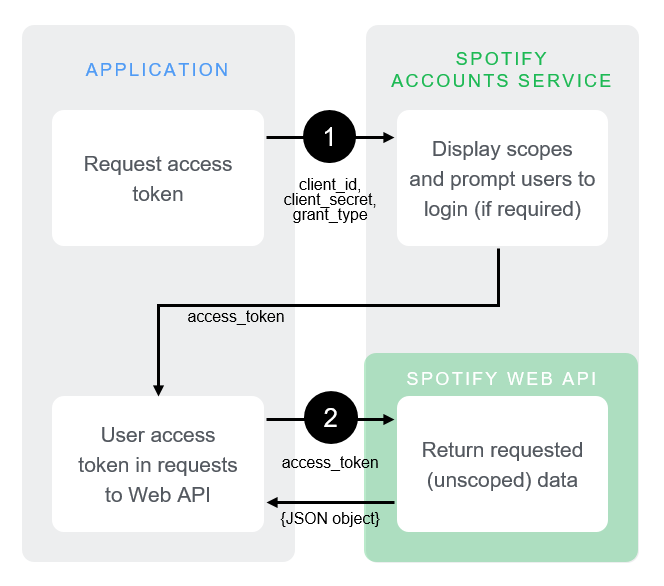
\includegraphics[width=7.5cm, height=7.5cm]{img/oauth.png},
\caption{oauth2}
\label{oauth2}
\end{figure}

\subsection{Sprint 8: Final touches and Spotify widgets}
In our final sprints we finished the final touches to the website e.g icons and animations and also added a Spotify widget to show what playlist the user has created.


\chapter{Technology Review}
In the following section, we will discuss the technologies used in the project, how we went about implementing them and the reasoning behind our decisions.

\begin{itemize}
  \item React
  \item Flask
  \item MongoDB
  \item Amazon Web Services
  \item TravisCI
  \item MochaJS
  \item Spotify API
  \end{itemize}

\section{React}
For developing the front-end of our application, we used React. React is a JavaScript library for creating responsive and elegant user interfaces. It is an open source technology and this was one of the 
driving forces which led us to choose it over other popular choices such as Angular, Vue.js or Ember. We were more comfortable working with open source software as we knew the documentation and help online would be much more reliable than traditional proprietary software.
React implements a component based architecture. This means that the user interface consists of multiple, abstracted \textbf{components} that each manage their own state and properties.
\par 
This component based architecture promotes re-use and efficiency as when the page loads, each component is loaded only once and is subsequently rendered and re-rendered accordingly when the data of that component changes. This means that in practice, instead of the user having to reload commonly rendered aspects of a web page such as
the footer and navigation bar every time they visit a new page, we only need to update the components that change. For example, if the user arrives at the home page of the website, they will load the navbar, footer and home components. On a traditional webpage, when visiting the register/login page they would have to reload the navbar and footer again. 
Using React, we were able to eliminate this shortcoming of traditional web design and only re-render what is required - the Login/Register forms.

This component based architecture also helped us to achieve one of our original goals of the webpage being fast and responsive to use.

This design approach implementing abstraction and re-use also means that it is easy and painless to share components with others and this greatly helped us rapidly develop the webpages in a clean and easy to understand manner. We were each able to work on separate components of the web page in parallel without massively conflicting with each others work.
We were then able to render these components depending on which RESTful route the user was on. We accomplished this using React-Router, a React library that enables the rendering of specific components on specific RESTful routes.

An example of this can be seen below

\begin{minted}{XML}
<Route path="/Register" 
  component={(props) => 
    <RegisterForm 
      createState={this.createState}>{props.children}
    </RegisterForm>}>
</Route>
\end{minted}

The above code means that when the user is on the route '/Register', render the component called 'RegisterForm'. We also create a state for this component and pass in the 'props' to this component.
'Props' refers to the parent component, which in this case is our Index page. We pass the current state of the parent component to it's child, RegisterForm.

As mentioned above, we used RESTful routes in our application. As such, we had needed a way to handle HTTP Requests. Unfortunately, unlike other popular front-end frameworks such as Angular, React does not include a HTTP Client to handle requests.
To combat this shortcoming, we researched a couple of popular JavaScript HTTP Libraries but ended up settling on of the most popular, Axios. 

Axios is a promise based HTTP client that works with nearly ever browser and has a host of features including automatically transforming requests into JSON, support for protecting against cross-side forgery attacks as well support for NodeJS. Axios was very simple to use and made handling HTTP Requests and Responses from our server painless and easy to handle.

\newpage

\begin{minted}{javascript}

// Perform Axios GET Request
// Sent to Flask server's route '/loginUser'
// Send our state variables captured by our handleChange function 
axios.post('/loginUser', {
    params: {
      email: this.state.email,
      password: this.state.password
    }
  })
  .then(function (response) {
    console.log("Server Response: " + response.status)
    if(response.status==200)
    {
      console.log("Successful Login!")
      self.handleSuccessfulLogin();
    }
    if(response.status==201)
    {
      console.log("Wrong login details!")
      self.toggleError();
      self.handleFailedLogin();
    }
    else
    {
      console.log("Server error!")
    }
  })
  .catch(function (error) {
    self.handleFailedLogin();
  });  
\end{minted}

As you can see from the code above, implementation is simple, logical and easy to understand.


\newpage\section{Flask}
In order to serve our React files, we needed a web server. We spent a lot of time researching this aspect of the application as we knew it would be a critical part and we did not want to regret our decision down the line. Some of the contenders included Ruby on Rails (Ruby), Django (Python) and 
Grails (Java). In the end, we decided on Flask as it suited our needs the most. Flask is 'microframework' written in Python. It's lightweight and get's it's 'microframework' name from it's lack of standard support for traditional functionality such as form validation, a database abstraction layer or object-relational mapping tools. Instead, these tools and libraries are provided by third parties. 
As a result of this architectural design choice, your resulting server can be custom-made to suit your specific needs with the least amount of bloat possible. This tied in nicely with our original goal of the application being fast and easy to use. The nature of Flask's architecture meant that we only had to include what we needed and no unused features and services was included.

Although originally conceived in 2010 as an April Fool's Joke \cite{FlaskOrigins}, Flask went on to be extremely popular being picked up by large corporations such as LinkedIn and Pinterest. A basic Flask application can be setup in as little as 7 lines 

\begin{minted}{python}
from flask import Flask
app = Flask(__name__)

@app.route("/")
def hello():
    return "Hello World!"

if __name__ == "__main__":
    app.run()
\end{minted}

One of the driving factors regarding our choice of Flask was that it is written in Python, a language none of us were hugely familiar with. We all thought it would be a good opportunity to learn a new language, especially since it is considerably
different to previous languages we had used such as C\# and Java.

Some of the Flask libraries we used in development of the application included 

\begin{itemize}
  \item Flask-PyMongo
  \item Flask-ByCrypt
  \item Flask-JWT
\end{itemize}

Flask-PyMongo enabled us to connect our MongoDB database with our Flask application in a simple and easy to use manner. 

Flask-ByCrypt helped us with the encryption of user's passwords before they were entered in the database upon registering as well as subsequent decryption of these passwords when attempting to log in.

Flask-JWT provided support for securing our RESTFul routes with JavaScript Web Tokens 

\section{MongoDB}
To satisfy our goal of an overall fast and efficient system, we wanted to make sure that access to the database was fast as well as secure. To satisfy this need, we chose MongoDB for our database.
We considered using an relational-style database such as SQL but we had used this technology many times before and we wanted to try something new. We also were aware that MongoDB used a document-style model to store information. This tied in nicely with our choice of Python as MongoDB's document-style of storing information is very similar to Python's 'dictionary' variable type.
It is also very similar to JSON Style documents which are passed in from our React front-end. Overall, this resulted in us being able toe easily pass the data between our React front-end, Flask back-end and our MongoDB database without having to hugely change the data at each step of the process.

As mentioned above, MongoDB uses a document-style model for storing information. This document style allows for many for many features such as 

\begin{itemize}
  \item Scalibility
  \item High performance
  \item Flexible and consistent
  \item Simple and powerful indexing tools
\end{itemize}

Another advantage of MongoDB is that like React, it's also open-source. This again played a large role in why we chose it as we knew that any questions or queries we might have about the technology would be easily answered online as developers of open-source software generally encourage this behaviour.

From our research, we also found that Mongo was considerably faster in general than traditional SQL databases, especially when the size of the tables/data was limited. However, I went delve into detail on this as the performance of this is discussed later in the System Evaluation chapter.

An example model of our MongoDB document we used can be seen below

\begin{minted}{javascript}
"_id": {
"$oid": "5c90d0d31fd421123063d92f"
},
"name": "Edward Eldridge",
"email": "steadyeddie101@hotmail.co.uk",
"password": {
    "$binary": "JDJiJDEyJDBlZWtUeTRMS0xQRnhFV0NGMU9vT08wb3Z5TTExOFdxTTP",
    "$type": "00"
},
"spotifyUsername": "Steadueddie",
"favArtist": [
    "Nujabes",
    "Kanye West",
    "Chief Keef",
    "Gotan Project",
    "Sia"
]
},
\end{minted}

In order for the application to function in the manner we intended, we needed to host the database somewhere remotely. We researched lots of ways of doing this but ended up settling on using a an Amazon Web Services Ubuntu Virtual Machine. The database was setup on a Ubuntu 18.04 system running on a virtual machine. The provided instance had no desktop or user interface so all the database set-up was done on the command line.
It was set up with security in mind, meaning a securely kept SSH key was needed to access the instance and a password was required to subsequently access the database. This meant the database and it's contents were kept secure. We had all experienced security issues with databases in previous projects, whether it was a ransom-ware attempt or deleting the contents of the database so this was a priority for us.


\section{Amazon Web Services}
Amazon Web Services, a subsidiary of the well known company Amazon, provides solutions to a vast range of cloud-computing problems. Some of these services include Elastic Beanstalk (for hosting websites), EC2 (for creating virtual machines) and they also provide their own database services if you don't fancy setting it up yourself.
As mentioned above, we used Amazon Web Services to host our MongoDB instance. However, we also used Amazon Web Services to host our actual Flask application so that it could be used by anyone, without the need to download and compile the source code.

To accomplish this task we used Amazon Web Services' \textit{Elastic Beanstalk} service. AWS describes Elastic Beanstalk as an 'orchestration' service. Essentially what this means is that they handle the large majority of the configuration, management and co-ordination required to keep a website hosted and up and running. To enable this, AWS provides a command line tool called AWS EB CLI. It's essentially a command line program that helps simplify creating, updating and monitoring your environments/applications from a local repository. 
AWS provides built in support for Flask applications so the setup was relatively simple. To further compliment our deployment, AWS provides support for Travis continuous Integration for seamless transition of code from a local repository to deployment.

We ensured that all our Amazon Web Services instances were on the EU-West server as we expected the large majority of our user-base to be based in Europe and this would enable better speeds and reliability. AWS also provides a lot of free services as our Ubuntu and Elastic Beanstalk instances were able to run for roughly 2 months before reaching the free tier. This is useful 
for people who might be curious as to what the process of hosting an application/setting up a database is like without having to pay excessive amounts of money. Once we reached our limit, we were able to supplement our credits with free credits provided by GitHub's Student Package. 

\section{TravisCI}
TravisCI or Travis Continuous Integration is a continuous integration tool that works in parallel with a GitHub repository. Continuous integration can be described as follows: Developers commit code to an online repository. Once this code has been committed, the code is then ran against automated tests to verify that it won't affect the overall stability and integrity of the system or application. Once this
code has passed the outlined tests, it's often passed onto to another service to be deployed such as Amazon Web Services or Heroku. In our case, we used TravisCI as our continuous integration tool. It's free, relatively easy to setup and works with any GitHub repository. To test our code before deployment, we used Mocha. Mocha is a Javascript testing framework that will be described in more detail below. Once the code passed the tests outlined by Mocha, it was automatically deployed to our AWS Elastic Beanstalk environment. This allows new features to be \textbf{quickly} and \textbf{safely} integrated with the live deployment of the application without 
the developers needing to fully understand the complete configuration of the Elastic Beanstalk environment. 

\begin{center}    
	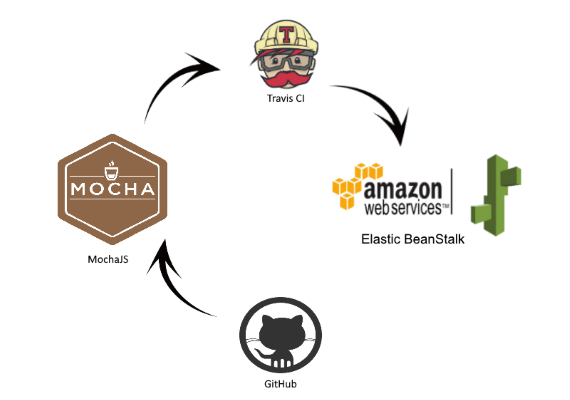
\includegraphics[width=14cm, height=12cm]{img/SDLC.png}
\end{center}


It also means that if there are bugs in the code, we are immediately notified by Travis via email whether or not the code managed to pass the tests. This means that bugs can be quickly squashed and less time is spent trying to figure out where the bugs came from and more time spent on developing actual new features. This ties in nicely with a lot of the core ideas behind one of the core concepts of the Agile software methodology - 'Working software is the primary measurement of progress.'

Below we can see a snippet of the Travis configuration file used to setup Travis with MochaJS and our Elastic Beanstalk environment.
\begin{minted}{java}
language: node_js

before_script: 
  - cd react-frontend 
  - npm install
  - npm run dev
  
script:
  - npm test

before_deploy:
  - npm run dev
  - cd ..

deploy:
  skip_cleanup: true
provider: elasticbeanstalk
  \end{minted}

\section{MochaJS}
Mocha describes it's self as a 'feature-rich testing framework' that runs on NodeJS. We were all relatively new to testing, having done only a small bit of unit testing with JUnit before. As such, we chose Mocha because it was easy to use and simple to integrate with Travis. 
Our tests were relatively simple as we expected many bugs throughout the development of the program and we wanted to ensure we didn't get bogged down on small bugs that wouldn't cause functionality problems but might stop our new features from being deployed.

\section{Spotify API}
One of the original goals set out by us when developing the application was that it was easy to use and integrated easily with existing technologies. To accomplish this goal, we chose to use Spotify to as both a music player and a music database as we suspected that a user likely to use our service would most likely already have a Spotify account. 
To facilitate the communication of our application and Spotify's music service, we needed an API. There are many different Spotify APIs available in a range of languages. We decided to use the Python Spotify library called 'Spotipy'. We chose to use the Python Spotify API as we thought it would integrate well with our existing Flask server, written in Python.

The 'Spotipy' module is not made by Spotify and as such is not officially supported. This meant that documentation for a lot of the functionality was lacking and was largely user-made. As a result, this hindered our progress significantly and it took an unplanned for amount of time to correctly setup the authentication that Spotify requires to make requests on behalf of the user. In hindsight, this was a mistake as we didn't realise that there was an official JavaScript API for Spotify. 
This would have likely been easier to use and less complicated to setup the authentication. As a result of this, we ended up re-writing a large majority of the Spotipy module to suit our needs. This resulted in us being able to achieve what we wanted but also some unexpected behaviour on the AWS deployment. Authentication was troublesome to setup on the AWS deployment as the module uses a Python's native HTTP MicroServer module in it's authentication process and it had trouble running consistently on our Elastic Beanstalk environment.

Despite these shortcomings, we were able to successfully use the Spotipy module to successfully manage and create playlists, give the user information about their own Spotify playlists as well handling any authentication required in this process.


\chapter{System Design}
We looked at different architectures for our web application and decided to use 3-tier architecture. In doing this we were able to separate the work between the group, purposely playing to each team members strengths. Utilizing a 3-tier architecture allowed us to comfortably work on one tier without impacting the other tiers directly. It proved especially useful when a update came out for the technology at a given layer, we were able to update that layer independently without trouble.\cite{3TierArchitecture}


We opted to utilise a 3-tier architecture consisting of the following components:

\begin{center}    
	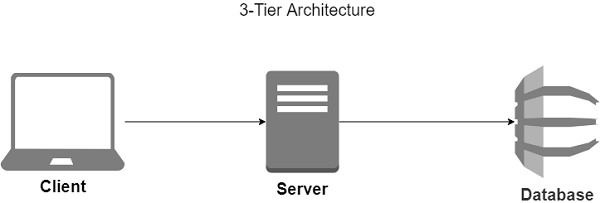
\includegraphics{img/3tier.png}
\end{center}

\subsection{React frontend (Client)}
The React front-end is what you see at the Presentation layer. This is what the user is interacting with on their own PC. On this tier input is received, and output is displayed.
We used ReactJS for the front-end as there is good support for it. A great thing about React is that you can create reusable UI components. React is good for its simplicity. It makes use of JSX syntax which allows you to produce React elements more intuitively, but still also allows you to write in plain Javascript.\cite{ReactDocumentation}


The React front end consists mainly of index.jsx and several separate component classes. The index page acts as an entry point and is the outermost component class in the React application. The index page handles the user logging in by passing in the email from the LoginForm component. Once the details are verified, the user is redirected to the Create page which contains the ArtistEnter component. The index page handles the user logging out by clearing the logged in state and redirecting back to the Home page. 
The index page is where the React components are rendered visually. The Home page components displayed consist of the NavBar, Carousel, Home, Get Started, and StickyFooter. 

\begin{center}    
	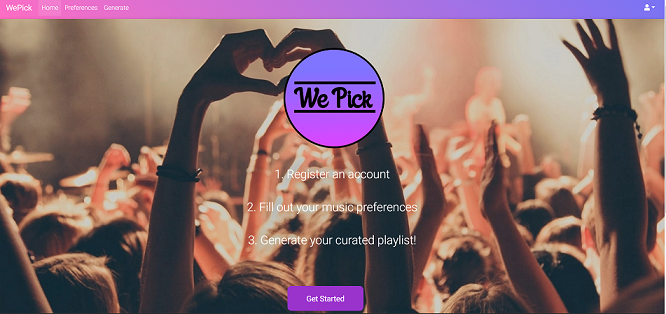
\includegraphics{img/WePickHome.png}
\end{center}
Here you can see the Home page as a new user will see it. You can see the NavBar at the top.
The background is a Carousel of images. The Get Started button is also visible.\newline


There is also a Create page which contains the ArtistEnter component along with Navbar and StickyFooter.\newline
The Register page consists of the RegisterForm component along with NavBar and StickyFooter.\newline
The Auth page is handled by the Auth component.\newline
The Login page consists of the LoginForm component along with with NavBar and StickyFooter.\newline


These components are then styled with multiple CSS files.\newline


The \textbf{LoginForm} component takes in the user’s email and password. Once the user clicks on the submit button, an Axios GET request is performed.It is sent to the Flask servers loginUser route.\newline
Below is an example of the axios request being sent to the /loginUser route\newline
\begin{minted}{Javascript} 
axios.post('/loginUser', {
params: {
email: this.state.email,
password: this.state.password
}})
\end{minted}

The \textbf{Logout} component simply clears any state held by its parent component and then redirects to the Home page.\newline

The \textbf{Home} component acts as the component between the NavBar, Carousel and StickyFooter components. The Home component is where the Get Started button is rendered.\newline

The \textbf{NavBar} component contains the navigation bar that is always rendered in the application. The user can follow the links on the NavBar to the Home, Preferences and Create pages respectively.\newline

The \textbf{Carousel} component is used to render an image carousel on the Home page. The carousel cycles through 7 different images and is a style choice which gives a more professional look to the application.\newline

The \textbf{DemoBlock} component renders the "Get Started" button which is visible on the Home page. The user can click this button and a particle effect animation will play with the button disintegrating. The user will then be taken to the Create page where they can enter parameters and generate a playlist.

The \textbf{Auth} component handles authorization.\newline

The \textbf{RegisterForm} component renders the form which is displayed to the user when they are registering a new account in the application. It takes in the user’s name, email and password. On submit the user’s information is routed to auth.\newline
Below is an example of how the users details are sent to authentication\newline
\begin{minted}{Javascript} 

handleSubmit(event){
console.log("Register successful.. Redirecting to authentication");

this.props.createState(this.state.name,
this.state.email, this.state.password);
		
this.props.history.push('/auth');
}
\end{minted}


The \textbf{ArtistEnter} component contains the form which allows the user to generate a play list based on their preferences. Once the user has logged in successfully, they can enter artists of their choosing. The user can move onto generating a playlist by submitting the form and adding the artists to their preferences.\newline
Below is an example of the ArtistEnter component on the /Create route found on the Create page.\newline
\begin{minted}{Python} 
<Route path="/Create" component={(props) => <ArtistEnter
 email={this.state.email}>{props.children}</ArtistEnter>}>
 
</Route>
\end{minted}



\begin{center}    
	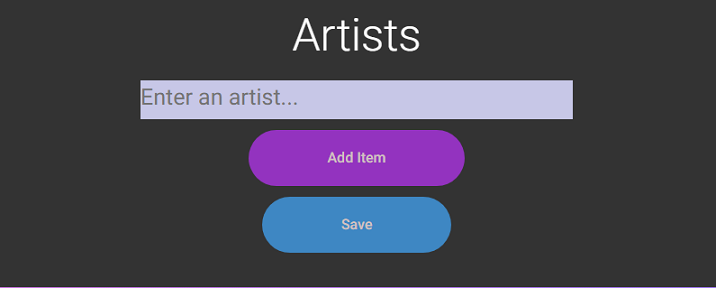
\includegraphics[width=12cm, height=5cm]{img/AddArtist.png}
\end{center}
Here you can see a close-up of where the user can enter an artist and add it to their preferences.\newline


The \textbf{Prefs} component is what is used to handle the user music preferences.\newline

The \textbf{StickyFooter} component renders the footer which is present on all pages of the application. The footer acts as a second navbar and contains information about the organization.\newline

\subsection{Python backend (Server)}
The python backend is what is present at the Application layer. This is the server which is made using flask and python. On this tier the logic is processed, and calculations are made.
\textbf{SpotipyAPI.py} is where the playlist generation is handled behind the front-end. When an artist is searched, a lot of information about the artist is returned i.e. Hometown etc.
The JSON data that is returned is where their artist ID is stored. This in-turn allows us to grab that artist ID and use it in generating the playlist.\newline

We make use of \textbf{OAuth 2.0}; this is the industry standard protocol for authorization. We use OAuth2 to authenticate the user through Spotify.\cite{OAuth2} When the user is trying to login to their account on our application, they are in turn brought to a login dialogue through their Spotify account. Once they have logged into Spotify they are authorized and can continue with our application.\newline

\begin{center}    
	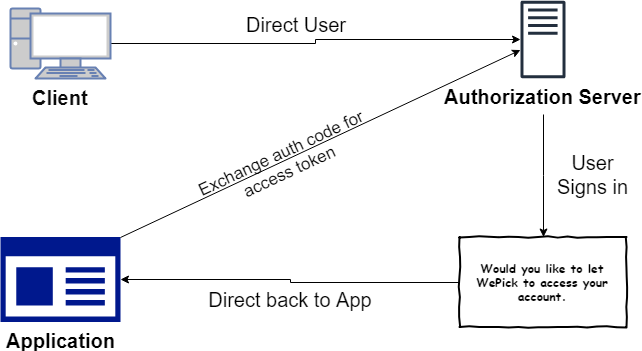
\includegraphics[width=14cm, height=10cm]{img/auth.png}
\end{center}
The user starts out by going to the application. The application then sends the user to the authorization server. The user logs in here and the authorization server sends the user back to the application. The application then makes a POST request to the authorization server to get an access token.\newline

\textbf{Application.py} is the main backend server content file in this project. This is where an instance of the DatabaseConnector.py is created. The Flask server is created here and pointed to the static file within the frontend to serve the HTML. The Mongo object is created here along with the Flask. The \textbf{getSpotifyUsernameByEmail()} function gets the Spotify username from the database. The default route of the application is here, and this is where the index.html file is rendered.\newline

The \textbf{CreatePlaylist()} function is where the playlist is generated. The function first gets the JSON data from the request and in turn gets the users from that JSON data. Any empty strings from the list of users are filtered out and the list of users is then converted into an array. The first user in the list is always the home user currently logged into the application.\newline

The favourite artists for all the users in the array are then retrieved from the database. The collection of artists is then combined into one large list and any duplicates of artists are removed. A random sample is taken from all the artists collected from the database.\newline 

The Spotify username is taken from the currently logged in user. Their username is passed onto authentication and a token is returned. The artist IDs of the random sample are retrieved and those IDs are passed on to the CreatePlaylist() function. A play list is then created.\newline

The \textbf{getArtistDB()} function sends a GET request to return the artists from the MongoDB database based on the users email address.\newline
Below is an example of this.
\begin{minted}{Python} 
@application.route('/getArtists', methods=['GET'])
def getArtistsDB():
artists = mongo.db.Users.find_one({'email':currentEmail},{'favArtist':1})
artists = artists['favArtist']
print(artists)

return json.dumps(artists)
\end{minted}

The \textbf{sendArtists()} function sends a POST request to update the users favourite artists.\newline
Below is an example of this.
\begin{minted}{Python}
@application.route('/UpdateFavArtists', methods=['POST'])
def sendArtists():
jsonData = request.get_json(force=True)
artistList = jsonData['dynamicList']
print(jsonData)
print("Inside fav aritst functon")
mongo.db.Users.update_one({'email':currentEmail},
                          {'$set' : {'favArtist' : artistList}})

return jsonify({'ok': True, 'message': 'artists updates'}), 200
\end{minted}

The \textbf{loginUser()} function handles the user logging into the application using a POST request. Once the login data comes in from the login form component the loginUser() function checks the JSON data, making sure it is in the correct format. The email is checked against the database to see if it is present. If this user’s email is present, the password is then checked to see if it is correct.  If the user’s password checks out, that password is deleted, and the user is given an access token in exchange. 
If, however the user does not have a registered email in the database, the user is notified on the client end. If the user does not supply the correct login details the user is notified also.\newline

The \textbf{showUser()} function uses a GET request to show specific details of a user. A query is taken from the HTTP request argument. The data is retrieved from the MongoDB database using this query and is displayed in JSON format.\newline

The \textbf{showAllUsers()} function is similar to the showUser() function  naturally. This function also uses a GET request and receives a query. It then queries the MongoDB database and retrieves the data. This data of all users is added to a list and is then printed out in the console.\newline

The \textbf{createUser()} function handles the user creating an account using a POST request. Once the user details come in from the form component the createUser() function validates the JSON data making sure it is in the correct format. The password is encrypted before it is inserted into the MongoDB database. Once the user details have been successfully added to the database the user on the client side is notified. If the user does not input parameters correctly, they receive an error message.\newline

The \textbf{deleteUser()} function uses a DELETE request to delete a user from the database. Once the user data is in the correct format and the user details are present, the record can be deleted from the database. If there is no such user present, then an error is thrown.\newline

The \textbf{updateUser()} function uses a PATCH request to update the user’s details. First the data is checked that it is in the correct JSON format. The MongoDB database is then queried to update the record if it is present, otherwise an error is thrown.\newline

The \textbf{auth()} function handles the Spotify authentication required , using a POST request. Once a GET request is received a token is generated in the browser. If the data is in the correct format, the token will be successfully generated and authentication will pass, otherwise it will fail.\newline
Below is an example of this.\newline
\begin{minted}{Python}
@application.route('/auth', methods=['POST'])
def auth():

jsonData = request.get_json()
print (jsonData)

scope = 'user-read-email user-read-private 
         user-read-playback-state 
         user-modify-playback-state 
         user-library-read playlist-modify-public'

if request.method == 'POST':
username = jsonData['spotifyUsername']

token = util.prompt_for_user_token(username,
                 scope,
                 client_id='e6b98ce6b2cf483c832c652aada81bea',
                 client_secret='5325fce64c6b4c4aad72b34029085111')
if token==None:
return jsonify({'ok': False, 'message': 'Authorization failed'}), 400
else:
return jsonify({'ok': True, 'message': 'Authorization Success'}), 200


\end{minted}


The \textbf{getSpotifyStats()} function uses a POST request to display the current users statistics. A user’s email is taken in, the stats are added to a list and displayed as JSON data.\newline


\subsection{MongoDB (database)}
The MongoDB is what is at the Data layer. On this tier data is stored and managed.\cite{MongoDBDocumentation} Once the database was set up, we wrote \textbf{DatabaseConnector.py}. We loaded in the IP address and password for the database from a config file found locally on the machine. Once the database was created, we could view the collection of users in the database.\newline

There are several getter functions written for this database which allows for basic functionality.

getUsersCollection(self) is a simple getter function which is performed on the database itself. The function returns the collection of users in the database.
getURI(self) function returns the Uniform Resource Locator of the database.
getClient(self) function returns the Client.
getDatabase(self) returns the Database.\newline

There are also functions which serve the database in handling user data.\newline

The \textbf{addUser()} function adds the id, name, favouriteArtists and favouriteSong of the user into the collection of users. This collection of users is in the database.\newline
The \textbf{showUsers()} function finds every user in the collection and displays them.\newline
The \textbf{deleteUser()} function takes in a user id and deletes a user from the user collection based on that id.\newline
The \textbf{showUsersFaveArtist()} function displays a user and their favourite artist depending on which user is shown from the collection.\newline

The MongoDB database is hosted remotely in the cloud using Amazon Web Services. The user on the client side should be able to access the application from any desktop. Therefore, it was necessary for us to host the application on a Ubuntu Virtual Machine. An SSH key is needed to gain access to the remote instance, and this SSH key is stored securely. A password is then also necessary to access the database. The configuration for the remote hosting was all done on the command line.\newline


\chapter{System Evaluation}
In this chapter, we will discuss many aspects of the software. We will break the evaluation down into 4 headings.
\begin{itemize}
  \item Robustness - How well the software can deal with problems, it's ability to handle change etc.
  \item Performance - Space and time complexity of the software, responsiveness etc.
  \item Security - How vulnerable is the application to attacks and security risks?
  \item Overall evaluation - Where the project succeeded/failed, limitations in our approach and technologies etc.
  \end{itemize}

  \subsection{Robustness}
  Robustness in regards to software can be defined as the ability of the software to cope with errors during execution and cope with erroneous input. Measuring the robustness of a system is difficult 
  as no system can be considered completely robust. However, there are certain methodologies and practices we can implement to increase the robustness of a system. {\textit{Behdis Eslamnour and Shoukat Ali}} discuss these metrics in their paper entitled {\textit{Measuring robustness of computing systems}}\cite{SoftwareRobustness}
  Some of these proposed metrics include
    \newline
    \begin{itemize}
      \item Error Handling/Error Catching
      \item Time between failures and time between recovery
    \end{itemize}

    \subsection{Error Handling}
    Error handling refers to how a system handles errors should they occur. This can be as simple as logging the error in the console to rolling back the system to a previous stable release.
    It is a vital aspect for any system from both the perspective of the user and developer. As a developer, implementing proper error handling and catching is an important aspect of development
    as it enables the developer to work more effectively and efficiently as less time is spent fixing and locating the cause of bugs if proper error handling is done pre-emptively.

    For the user, it's vital that error handling is done correctly as incorrect error handling can have a significant impact on the end-users experience of the system/software. For example, if a user
    attempts to login to a system and their login details are incorrect, a meaningful way of handling this error would be to notify the user that their login details are incorrect. If this is not done, 
    the end user won't understand what's happening and why they can't use the system and as a result of this will become frustrated/unhappy with the service. As such it's important to make sure any critical
    problems such as this are caught and handled in an appropriate manner. However, it's also important to remember that complete robustness can not be achieved and as such one must try and figure out the 
    most important and likely errors to handle. When making these decisions, one can consider many factors when deciding what errors to handle such as the risk of not handling the error (application crashing, unexpected behaviour, potential security risk, loss of data etc.)
    , how much time will be required to handle the error and the likelihood of the error occuring. However, as mentioned above complete robustness can not be achieved as to even consider the above factors,
    one must have the foresight to see that the error will occur in the firstplace.

    Some examples include of error-handling include \textit{Error boundaries} in React, \textit{Try/Catch/Raise statements} and \textit{Schema validation} in MongoDB.

    \begin{itemize}
      \item Error Boundaries - Error boundaries are React components that catch JavaScript errors anywhere in their child component tree, log those errors, and display a fallback UI instead of the component tree that crashed.
      \item Try/Catch/Raise statements - These commonly found in most programming languages and Python is no exception. We used these to catch certain errors such as HTTPErrors, null value errors, MongoDB errors and many others.
      \item Schema Validation - To ensure the data being passed into the Mongo database was in the correct format, we used a JSON Schema to validate our inputs against before passing it to Mongo. In the below example, we can see that for a user 
      to be validated correctly, the minimum required properties are an email and password. This ensures that user's cant create accounts without these two required properties.
      \begin{minted}{JSON}
      user_schema = {
        "type": "object",
        "properties": {
            "name": {
                "type": "string",
            },
            "email": {
                "type": "string",
                "format": "email"
            },
            "password": {
                "type": "string",
            },
            "spotifyUsername": {
                "type": "string",
            },
          
        },
        "required": ["email", "password"],
        "additionalProperties": False
      }
      \end{minted}
      
    \end{itemize}

    \subsection{Time between failures and time between recovery}
    Time between failures and time between recovery are too very useful metrics in determining the robustness of a system. Systems that have a short mean time between failures and mean time between recovery
    either have excellent error handling or are designed in such a way that errors do not occur frequently. A good way of measuring this could be 
    the downtime of your application over the course of a year. For example, on average, the top 50 e-commerce websites experienced 99.03\% uptime. Over a year, 99.03\% uptime would result in 3 days 15 hours and 39 minutes of downtime. 32 of
    these websites experienced 99.99\% uptime. 9 out of 10 of users encountering a website that is not up will choose to use a competitors website \cite{WebsiteDowntimeStats}. From these statistics, we can see that time between failures anre time between recovery are extremely important aspects to 
    any system/application. As such, they can be very helpful metrics when trying to measure the robustness of an application. 

    In regards to WePick's failure and recovery time, since the project was hosted on AWS' Elastic Beanstalk, there have been little to no outages as due 
    to the continuous integration solution integrated upon deployment, it was not possible for broken code to be deployed as any code proposed to be deployed had 
    to first pass tests that were outlined by Travis CI and any problems that did arrive were dealt with quickly as Travis instantly notified us of any problems which we were 
    able to fix quickly and promptly.

    \subsection{Performance}
    When planning and designing the project, one of our main aim's was that we wanted the project to perform operations and tasks quickly as well as being responsive to user input. Taking these considerations into account, we choose
    Python and MongoDB for our backend as they are generally considered lightweight and easier to handle performance than say something like Java. We chose React for the front-end of the application as React is well known for it's performance and
    responsiveness. This generally comes from the fact that React applications usually implement a single page design. React works by creating multiple components that can be re-used multiple times in the application. For example, in our 
    application, instead of creating multiple pages with the same code (Navbar, Footer, Forms etc.), we can create seperate components for each of these items and only re-render what is required. So if the user needs a different form only that form will
    be re-rendered and the Navbar and Footer don't need to be re-rendered This choice of technology helped us achieve our overall goal in regards to perfromance and I think it was a good choice.

    Our choice of MongoDB as a database was also important to the overall perfromance of our application as MongoDB is considered much faster than SQL \cite{SQLvsNOSQLPerformance} and other relational databases in certain scenarios. This is because of it's non-relational, no-SQL way of storing data.
    Instead of storing data in rows, columns and tables, Mongo works by using a document style architecture. These documents are structured similarly to a JSON document and as such are easy to extract data from and manipulate without navigating through 
    large sets of data like you would in a traditional SQL database. Generally, this performance increase can be seen most when you start to scale up the size of your database. For our application, it was important to be able to access user's favorite artists
    quickly so that they didn't have to wait a long time to generate a playlist.  

    \begin{center}    
      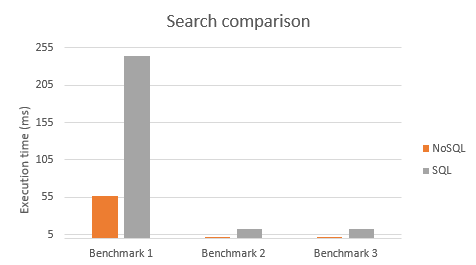
\includegraphics{img/SQLvsNOSQL.png}
    \end{center}

    From the above graph, we can see that when performing a search in the database, NoSQL databases like Mongo are considerably faster than a traditional SQL database \cite{SQLvsNOSQL}

    \subsection{Security}
    Securit was an important factor for us to consider when designing and creating the application as we had all experienced problems with group projects in the previous year. For example, many students dealt with problems where database tables were wiped and/or hijacked and held ransom
    to the owners. As such, we did not want to deal with such problems and thought it would be a good oppurtunity for us all to learn a bit more about how one goes about securing an application in a real world context. We also wanted user's information to be secure and not easily accessible by anyone.
    
    To ensure our RESTful routes were not accessible to anyone, we implemented JWT Tokens into our application. A JWT Token or JSON Web Token is an open-standard that defines a way for securely transmitting and verifiying information between systems.
    JWT's are signed using a secret key or a public/private key using RSA encryption.
    
    The way this ends up working in the application is as follows. When the user successfully logs in, a JSON Web Token is generated and each subsequent request
    made by the user will include that web token. Setting up the system in this way means that to perform a HTTP request on one of our many RESTFul routes, the user first has to 
    verify that they are an authenicated user. This prevents from people performing actions on routes that they should not have access to. 

    A traditional JSON Web Token consists of a Header, Payload and Signature in the following format 

    \begin{minted}{JSON}
      header.payload.signature
    \end{minted}

    The header details what type of token is being sent and the algorthim used to generate the token.
    The payload contains the information about the person sending the token and what they would like to do.
    The signature is essentially an your header and payload encrypted and is used to verify the payload wasn't altered during transit as well as verifying the sender is who they say they are.
    
    An example token can be seen below

    \begin{center}    
      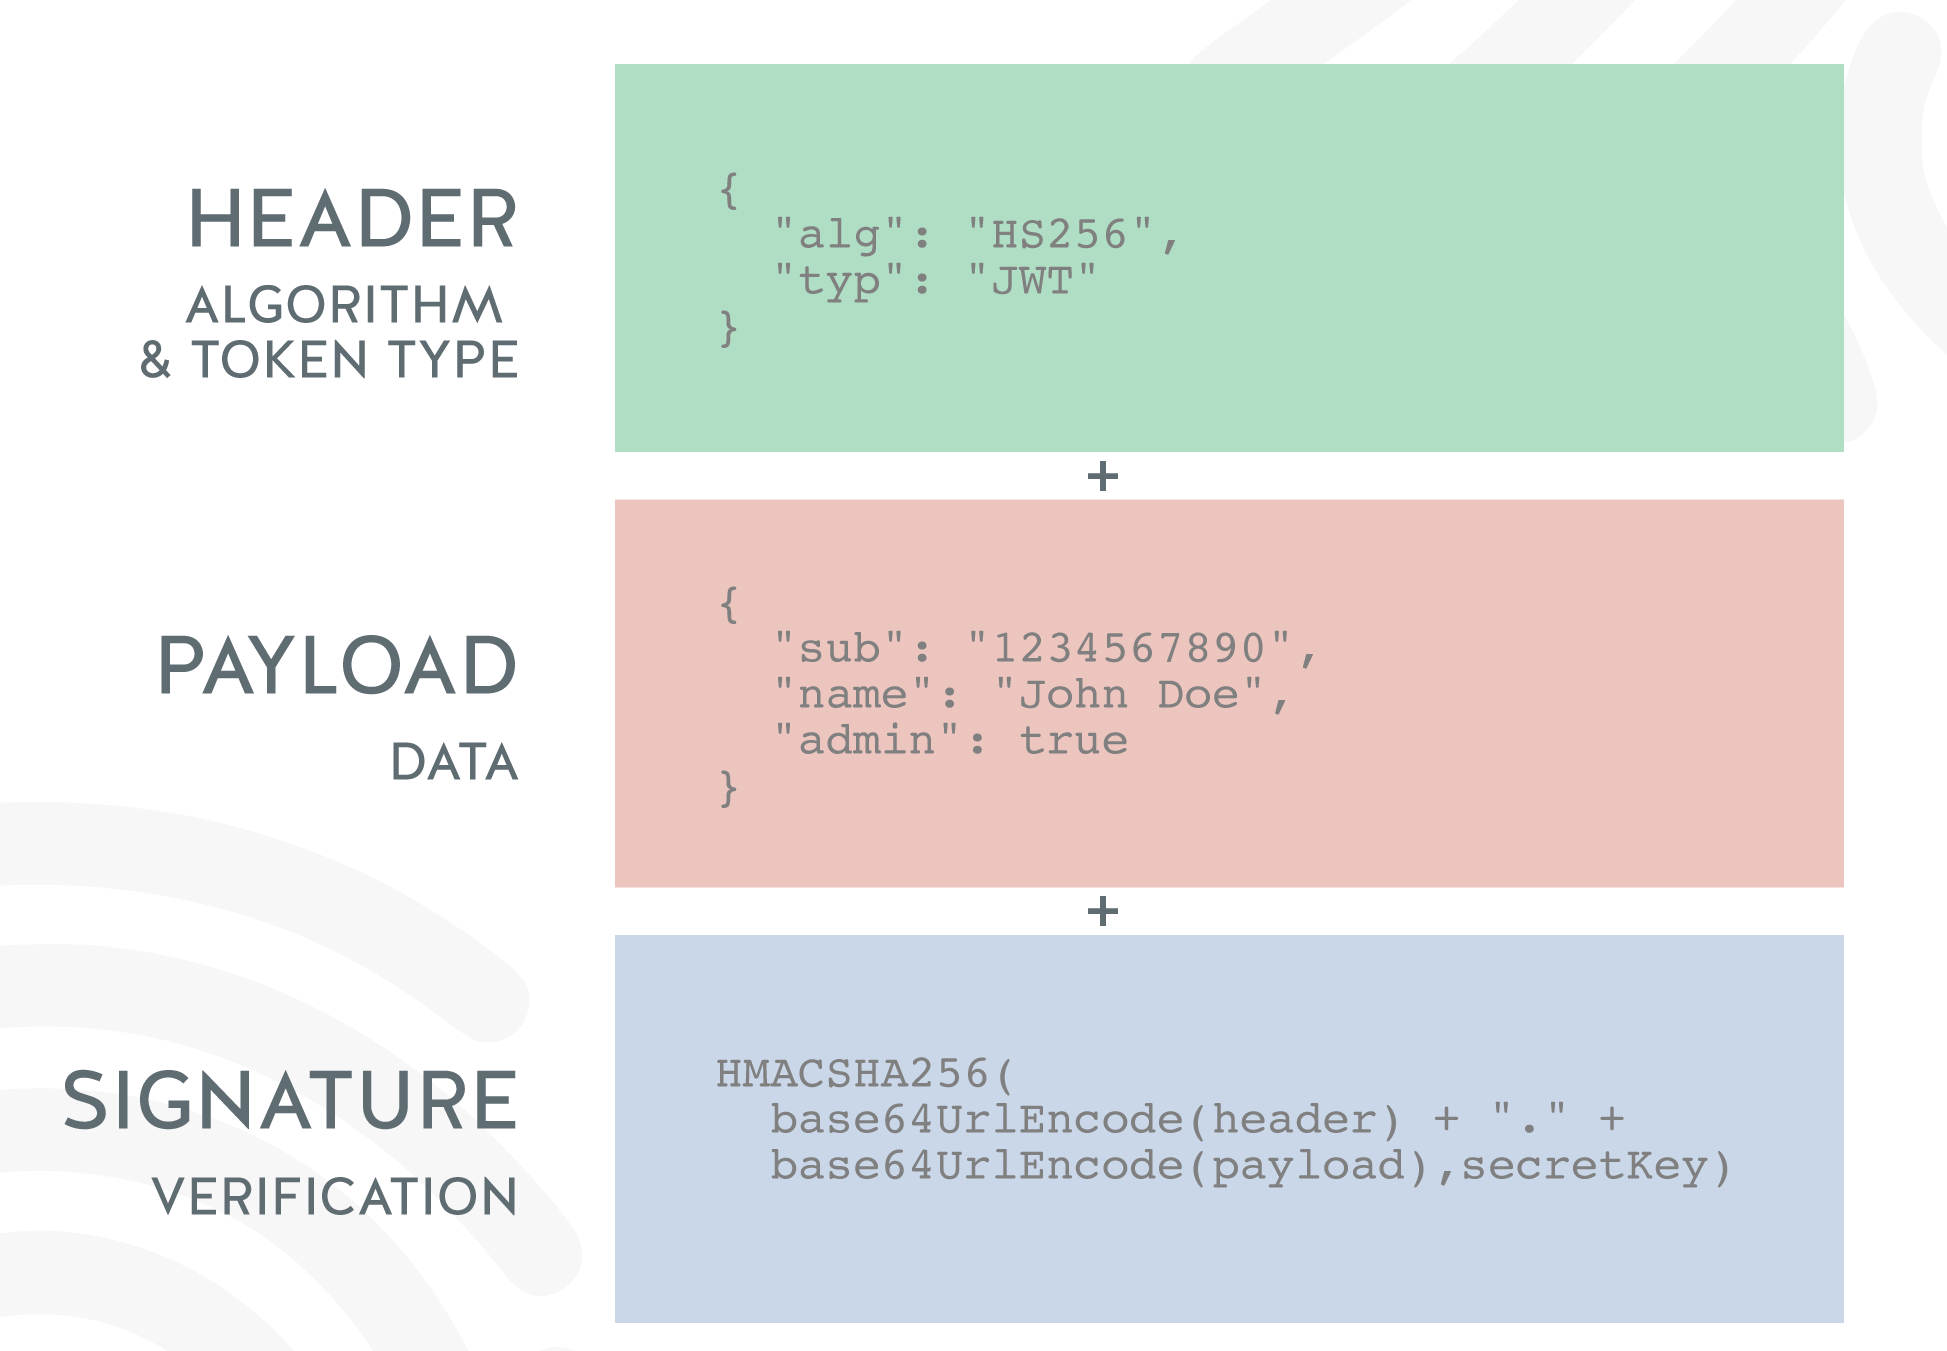
\includegraphics[width=15cm, height=10cm]{img/JWTTokens.png}
    \end{center}

    To implement this technology in our application, we used Flask-JWT, a simple Python library that provides JWT Support for Flask applications.
    A simple example of how this technology was implemented can be seen below.

   
    \begin{minted}{Python}
      @application.route('/refresh', methods=['POST'])
      @jwt_refresh_token_required
      def refresh():
          current_user = get_jwt_identity()
          ret = {
                  'token': create_access_token(identity=current_user)
          }
          return jsonify({'ok': True, 'data': ret}), 200
      
      @jwt.unauthorized_loader
      def unauthorized_response(callback):
          return jsonify({
              'ok': False,
              'message': 'Missing Authorization Header'
          }), 401
    \end{minted}

    As well as ensuring API calls were authenicated, we also made sure that our database and user information was secure. A secure admin account was created on the database, requring a password to perform any actions in the databse.
    This way, no operations could be performed on the database without knowing both the IP address of the server the database was hosted on and the password required to gain access. These two important pieces of information were known only to us and 
    weren't available anywhere else. 

    We also made sure that any important user information such as passwords were encrypted before being entered into the databse.
    For this, we used another Python library for Flask entitiled Flask-Bycrypt. Using this library, we can generate a hash of the user's password and store this in the database instead of storing their password in plaintext. Then, when checking if 
    the user's login details are correct, we compare the generated hash of the passwords instead of the actual passwords themselves. This enables a secure login scenario and prevents passwords being revelead to anyone.

    To improve overall security, we also chose to host our application on a different instance than our database. This meant that if one were to be compromised in any way, it would prevent the other in turn being compromised.

    \subsection{Improving Security}
    \subsubsection{HTTP/HTTPS}
    One shortcoming of our project is the lack of a secure Hyper Text Transfer Protocol (HTTPS). HTTP can be described by Mozilla's standards \cite{HTTPviaMozilla} as an application-layer protocol 
    for transmitting data and documents. It was originally designed for communication between web browsers and web servers but it has since exceeded it's original purpose. It follows a client/server model. The client makes a 
    request to establish a connection and waits for a response from the server. Despite this however, it is a \textbf{stateless} protocol. This means that once communication between server and client, the server forgets all information regarding
    the communication. It can be used on any reliable transfer layer such as TCP/IP or UDP.

    The difference between HTTPS and HTTP is that HTTPS is considered 'secure' where HTTP is not. Essentially, the difference between the two can be illustrated cleary in the following diagram.

    \begin{center}    
      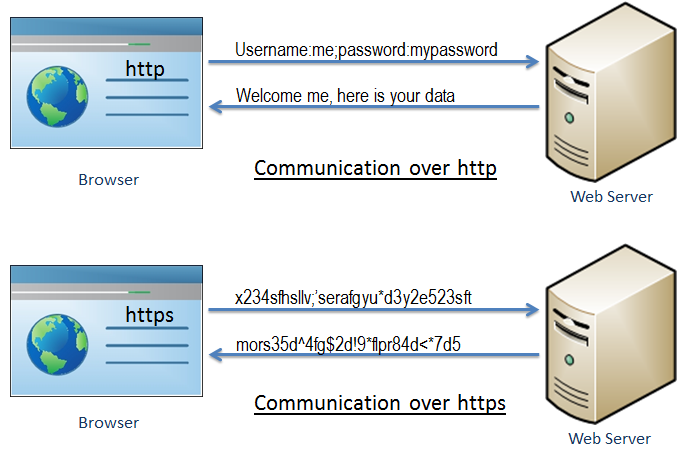
\includegraphics[width=13cm, height=10cm]{img/HTTPS.png}
    \end{center}

    In standard HTTP, the information is transmitted in hypertext format whereas with HTTPS, the information is first encrypted before sending the information.
    The issue with standard HTTP is that the data is transmitted in plaintext. This means that anyone who can 'see' the data or is monitoring the network can potentially intercept this data and/or modify it before being passed on to the server. This can 
    lead to serious security issues. This could be potentially devestating to an application/system that relies on sensitive data such as passwords or bank/card details.

    HTTPS guarantees that even if the message is intercepted, it would be of no value as it is encrypted. HTTPS provides these guarantees using a security standard known as SSL or Secure-Socket Layer.
    SSL is a standard for establishing an encryped link between a client and server. To first use SSL, one must aquire an SSL certificate. These certificates are small files that bind a domain name/IP address/hostname to an organizational identity and location.

    \subsubsection{But who exactly has the authority to issue these certificates and how can we trust them?}
    To issue SSL certificates and guarantee their authenticity, one must become a Certificate Authority. 
    This title is usually limited to private companies and governments that have proven that the certificates they issue are secure. The more secure certificates they authorize, the more certificates they are able to distribute. 
    This means that when aquiring an SSL certificate, you can guarantee it's authenticity. A certified certificate should contain your domain name, company name, address, city, state, country. It also contains an expiration date upon which the certificate must be renewed as well as the Certificate Authority that issued the certificate in the first place.
    All these factors provide some kind of accountability in regards to the certificate if something were to go wrong. Expiring certificates is a common occurence, even for large companies. According to GlobalSign \cite{GlobalSign}, between just October 2017 and February 2018, large organizations such as LinkedIn, PokemonGO the British Conservative Party and astonglishly The White House 
    have all let their SSL certificates expire. Any users arriving on these websites would have been instantly greeted with a warning that these websites are not secure and sensitive information could have possibly been leaked in the process. For something like a goverment website, this kind of behaviour is a perfect example of why we have SSL and HTTPS in the first place and why it's vital that these systems are maintained and updated.

    \subsubsection{How does SSL work?}
    Let's use a traditional client/server architecture as our example. The browser/client connects to the server secured with SSL. The server will then prompt the client to identify itself.
    The server then sends a copy of it's SSL certificate. These certificate is then verified by the client. \cite{SSLExpired} If verification is successful and the client is comfortable sending messages, it sends a response to the server which consists of a digitally signed acknowledgement which initiates an SSL encryped session.
    Any data exchanged between these two parties is now sent over the Secure-Socket Layer established by the client/server.


    \subsubsection{Benefits of SSL/HTTPS}
    We can describe the overall benefits of SSL/HTTPS as the following

    \begin{itemize}
      \item Utilize HTTPs, which elicits a stronger Google ranking.
      \item Create safer experiences for your customers.
      \item Build customer trust and improve conversions.
      \item Protect both customer and internal data.
      \item Encrypt browser-to-server and server-to-server communication.
      \item Increase security of your mobile and cloud apps.
    \end{itemize}

    \subsubsection{Why didn't we implement SSL/HTTPS?}
    Due to the nature of aquiring an SSL certificate, one usually has to purchase a certificate and pay a yearly fee for using it. We made a decision based on the information stored by our application and by factoring in the cost, decided that we didn't think it would be critical if HTTPS wasn't implemented.
    We understand it makes our application insecure, but we also understand why it makes it insecure and how this could be dealt with appropriately in future projects.


\chapter{Conclusion}

\subsection{Original Idea vs. Actual Implementation}
Our original idea/plan for this project was to create an application that created curated playlists based off multiple user's music preferences. This was our original idea before we had chosen any technologies or done any kind of design. Limiting the scope to this simple statement, I feel like we achieved our original goal that we set out in late September.
Up to 6 users can go on our website, create an account, enter their music preferences and create a curated playlist of music based on their and their friends preferred music. We also wanted the website to be simple and intuitive to use without the user feeling overwhelmed or confused as the original purpose of the program was simple and as such the website should be simple to use. \par
We focused heavily on this as we all felt like that websites can be extremely overbearing and complicacted when sometimes the user just wants to perform a simple task and having to go through hoops to perform this simple task can be extremely frustrating.

\subsection{Learning Outcomes}
At the end of our app development I can see that we learned a huge amount, I would even go as far as saying that it was a fantastic opportunity to see how easy it is to learn new technologies when you are a part of a team.
\par
We now have gained huge experience in coding in React, a very popular industry standard front-end framework. We also now have a lot of experience in deploying apps and the configurations it takes to get an app deployed on a web service such as Amazon Web Services. It was also very interesting to learn about how HTTP methods are used so widely to manipulate data from a front-end service to a back-end service. One of the things we found most interesting was how important it is to perform testing and continuous testing all throughout your project, this allowed us to see mistakes we were making all throughout the project rather than just at the end where it may have been a huge effort to fix.
\par
All in all though it were a very difficult project but the knowledge and expereience we gained while dveloping it was well worth it.

\subsection{Shortcomings/Oppurtunities}
In the future we would love to get our web app fully deployed to a top tier web hosting service to make it available to as many users as we wanted but as currently we don’t have the capital or the time to achieve this due to our exams. But we feel this web application has the potential to be an essential app that a huge amount of people would benefit from every day. We would also love to further develop the web application to convert it to both Android/iOS applications, so we can make it available to a greater proportion of people.

\subsection{Closing Statement}
In the end, we had a huge amount of enjoyment working on this web application. Although it was a huge amount of work, we are extremely happy with the professional standard of our application and the overall look and feel of it. It also has shown to us how much more enjoyable it is to work on a project with a team rather than on our own as it is far easier to distribute the work load and ask each other for help when working as part of a team. 
\par
Although we started this project as good friends, the whole journey has brought the three of us together as a group and the experience we gained developing this project will stand for us as we advance through our careers.

\subsection{Acknowledgements}
We would like to wish a huge thank you to our project supervisor Martin Kenirons for his continued help and support throughout the year. Without his continued help and support, this would have been a far more difficult project. We would also like to thank John Healy, Head lecturer of the Applied Project and Minor Dissertation module.


